\documentclass[alternative-exam.tex]{subfiles}
\begin{document}

\chapter{Een ei bakken}
\section{Vraag}
Als student krijg je tijdens het werken wel eens zin in spek met eieren. Als luie student vind je het al een opgave om naar de keuken te gaan om het eitje te bakken. Voor je vertrekt naar de keuken wil je al precies weten welke stappen je moet ondernemen, zodat je zeker niet teveel moeite doet. Met het STRIPS planning algoritme kan je dit probleem oplossen.

\subsection{Begin- en Eindsituaties}
\begin{figure}[H]
\centering
\begin{tabular}{|c|c|}
    \multicolumn{2}{c}{I}\\
    \hline
    if & -\\
    \hline
    add & In(Kamer)\\
        & Vrij(Pan)\\
    \hline
    del & -\\
    \hline
\end{tabular}
\hspace{0.25 cm}
\begin{tabular}{|c|c|}
    \multicolumn{2}{c}{F}\\
    \hline
    if & In(Kamer)\\
    & heeft(Maaltijd)\\
    \hline
    add & -\\
    \hline
    del & -\\
    \hline
\end{tabular}
\caption{begin- en eindtoestand}
\label{ienf}
\end{figure}
Figuur \ref{ienf}, toont de begintoestand en de gewenste eindtoestand. In de begintoestand zit de student aan zijn bureau in zijn kamer en heeft hij honger. In de eindtoestand zit de student weer aan zijn bureau en heeft hij een bord met gebakken spek en eieren.
\subsection{Acties}
Het hele proces kan beschreven worden een door aantal acties die de student kan ondernemen.
\begin{itemize}
\item
De student kan naar de keuken wandelen en terug. In figuur \ref{keuken} staan de overeenkomstige acties beschreven.
\begin{figure}[H]
\centering
\begin{tabular}{|c|c|}
    \multicolumn{2}{c}{H}\\
    \hline
    if & In(Kamer)\\
    \hline
    add & In(Keuken)\\
    \hline
    del & In(Kamer)\\
    \hline
\end{tabular}
\hspace{0.25cm}
\begin{tabular}{|c|c|}
    \multicolumn{2}{c}{T}\\
    \hline
    if & In(Keuken)\\
    \hline
    add & In(Kamer)\\
    \hline
    del & In(Keuken)\\
    \hline
\end{tabular}
\caption{van en naar de keuken wandelen}
\label{keuken}
\end{figure}
\item 
In de keuken kan de student koken en alle overeenkomstige acties daarvoor staan beschreven in figuur \ref{koken}.
\begin{figure}[H]
\centering
\begin{tabular}{|c|c|}
    \multicolumn{2}{c}{NeemEi (NE)}\\
    \hline
    if & In(Keuken)\\
    \hline
    add & Heeft(RauwEi)\\
    \hline
    del & -\\
    \hline
\end{tabular}
\hspace{0.25cm}
\begin{tabular}{|c|c|}
    \multicolumn{2}{c}{NeemSpek (NS)}\\
    \hline
    if & In(Keuken)\\
    \hline
    add & Heeft(RauwSpek)\\
    \hline
    del & -\\
    \hline
\end{tabular}
\\\vspace{0.25cm}
\begin{tabular}{|c|c|}
    \multicolumn{2}{c}{BakEi (BE)}\\
    \hline
    if & In(Keuken)\\
    & Vrij(Pan)\\
    & Heeft(RauwEi)\\
    \hline
    add & Heeft(EiKlaar)\\
    \hline
    del & Heeft(RauwEi)\\
    \hline
\end{tabular}
\hspace{0.25cm}
\begin{tabular}{|c|c|}
    \multicolumn{2}{c}{BakSpek (BS)}\\
    \hline
    if & In(Keuken)\\
    & Vrij(Pan)\\
    & Heeft(RauwSpek)\\
    \hline
    add & Bakt(Spek)\\
    \hline
    del & Heeft(RauwSpek)\\
    & vrij(Pan)\\
    \hline
\end{tabular}
\\\vspace{0.25cm}
\begin{tabular}{|c|c|}
    \multicolumn{2}{c}{DraaiSpekOm (DSO)}\\
    \hline
    if & In(Keuken)\\
    & Bakt(Spek)\\
    \hline
    add & Heeft(SpekKlaar)\\
    & Vrij(Pan)\\
    \hline
    del & Bakt(Spek)\\
    \hline
\end{tabular}
\hspace{0.25cm}
\begin{tabular}{|c|c|}
    \multicolumn{2}{c}{LegOpBord(LOB)}\\
    \hline
    if & In(Keuken)\\
    & Heeft(SpekKlaar)\\
    & Heeft(EiKlaar)\\
    \hline
    add & Heeft(Maaltijd)\\
    \hline
    del & Heeft(SpekKlaar)\\
    & Heeft(EiKlaar)\\
    \hline
\end{tabular}
\caption{koken}
\label{koken}
\end{figure}
\end{itemize}

\section{Modeloplossing}
\subsection{Establishes/Threathens-graaf}
\begin{figure}[p]
\centering
\caption{Establishes/Threatens-graaf}
\label{strips_1}
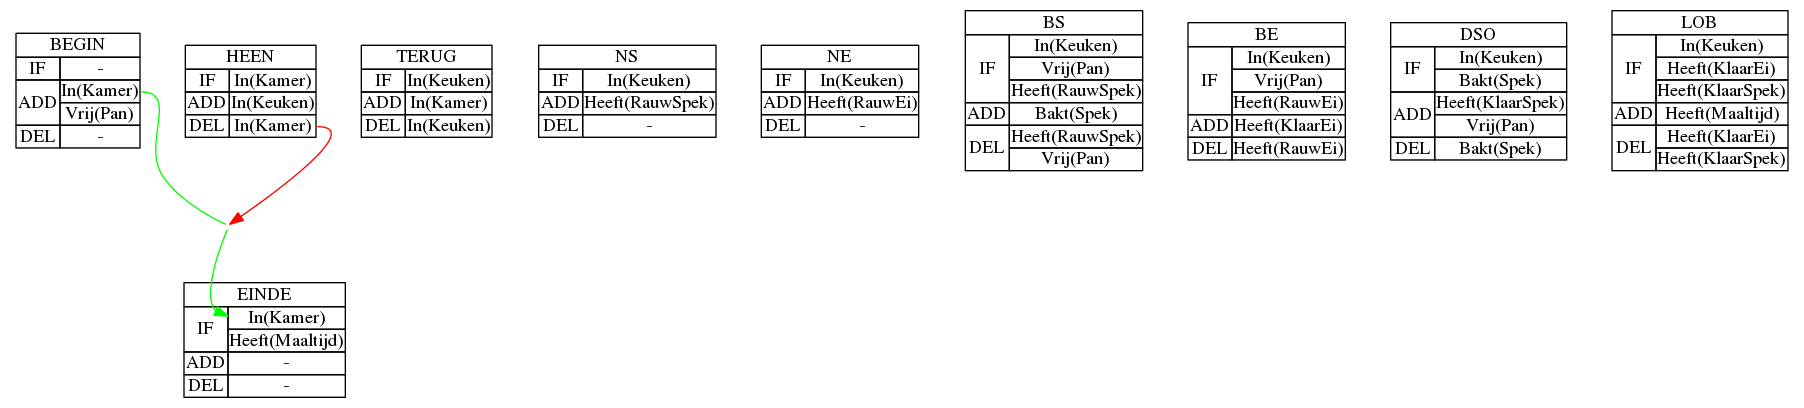
\includegraphics[scale=0.25]{resources/graphs/strips_1.png}
\end{figure}
In het eerste deel van de oplossing stellen we de graaf op met alle 'establishes' en 'threatens' relaties. Dit gebeurt als volgt. We beginnen met de begin en de eindsituatie te tekenen. Nu gaan we alle precondities voor de eindsituatie af. Voor elke operatie die we toevoegen gaan we diepte eerst, recursief alle precondities af. $In(Kamer)$ is al waar bij het begin. We proberen aan $Heeft(Maaltijd)$ te voldoen door $LOB$ toe te voegen. Om aan de preconditities van $LOB$ te voldoen voegen we eerst $HEEN$ toe (om aan $In(Keuken)$ te voldoen). We zien nu dat $DEL In(Kamer)$ van $HEEN$ $ADD In(Kamer)$ bedreigt. Dit betekent dat $HEEN$ ofwel voor het begin zou moeten gebeuren, ofwel na het einde. Omdat dit beide niet kan verwijderen we de 'establishes' boog van $BEGIN$ naar $EINDE$ (Deze boog is wel getekend voor de duidelijkheid). Deze procedure zetten we verder tot aan alle precondities van $EINDE$ voldaan is en we een graaf bekomen zoals in figuur \ref{strips_1} \footnote{Ter informatie: De uiteenzetting van de procedure is niet gevraagd.}.

In de graaf van figuure \ref{strips_1} zijn de groene bogen de 'establishes' bogen. Ze houden in dat de eigenschap bij het vertrekpunt ervoor zorgt dat aan een eigenschap bij het eindpunt voldaan is. De operatie waar de boog begint moet dus voor de operatie aan het eind van de boog plaatsvinden.
De De rode bogen zijn de 'threatens' bogen. Deze betekenen dat de eigenschap bij het vertrekpunt de eigenschap bij het vertrekpunt van de boog waar hij naar wijst ongedaan maakt. De operatie waar de rode boog begint moet dus ofwel voor het vertrekpunt van de boog waar hij naar wijst plaatsvinden, ofwel na het eindpunt.
\subsection{Before-graaf}
\begin{figure}[H]
\centering
\caption{Before-graaf}
\label{strips_2}
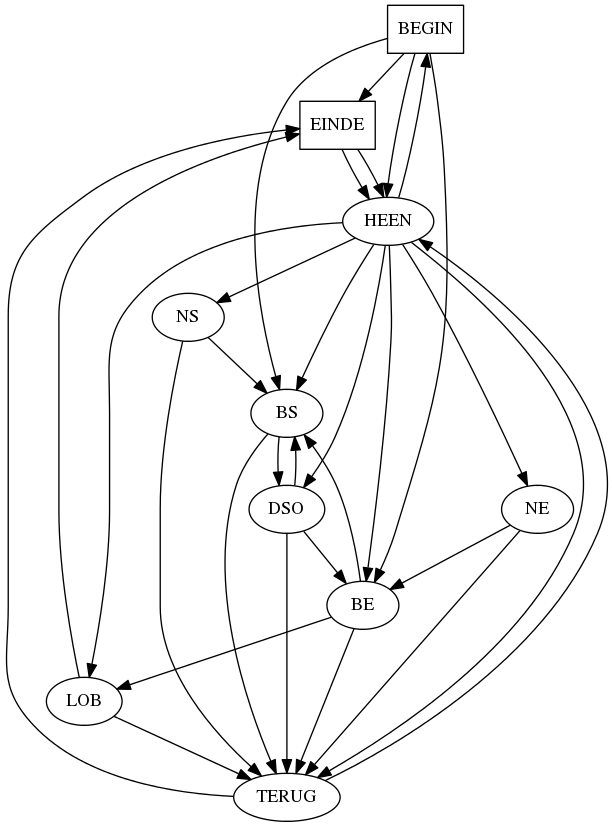
\includegraphics[scale=0.3]{resources/graphs/strips_2.png}
\end{figure}
In figuur \ref{strips_2} is de graaf getekend met alle 'before'
-relaties. We kunnen nu de mogelijke plannen opstellen. 

In elk plan moeten we eerst naar de keuken gaan en op het einde het ei en het spek op een bord leggen, waarna we terug naar de kamen gaan. Er zijn echter een aantal mogelijke plannen omdat we daartussen kunnen koken in een aantal mogelijke volgorden.

Het is makkelijk in te zien dat het niet uitmaakt of we eerst het ei bakken en daarna het spek. Bovendien maakt het niet uit of we eerst het ei uit de koelkast nemen of eerst het spek. We kunnen zelfs eerst het ei uit de koelkast nemen, dan het spek, eerst het spek bakken, en daarna pas het ei. Alle mogelijkheden zijn hieronder samengevat.
\[
\begin{array}{c}
BEGIN \rightarrow HEEN \rightarrow NE \rightarrow NS \rightarrow BE \rightarrow BS \rightarrow DSO\rightarrow LBO \rightarrow TERUG \rightarrow EINDE\\
BEGIN \rightarrow HEEN \rightarrow NE \rightarrow NS \rightarrow BS \rightarrow BE \rightarrow DSO\rightarrow LBO \rightarrow TERUG \rightarrow EINDE\\
BEGIN \rightarrow HEEN \rightarrow NE \rightarrow NS \rightarrow BS \rightarrow DSO \rightarrow BE\rightarrow LBO \rightarrow TERUG \rightarrow EINDE\\
BEGIN \rightarrow HEEN \rightarrow NE \rightarrow BE \rightarrow NS \rightarrow BS \rightarrow DSO\rightarrow LBO \rightarrow TERUG \rightarrow EINDE\\
BEGIN \rightarrow HEEN \rightarrow NS \rightarrow NE \rightarrow BE \rightarrow BS \rightarrow DSO\rightarrow LBO \rightarrow TERUG \rightarrow EINDE\\
BEGIN \rightarrow HEEN \rightarrow NS \rightarrow NE \rightarrow BS \rightarrow BE \rightarrow DSO\rightarrow LBO \rightarrow TERUG \rightarrow EINDE\\
BEGIN \rightarrow HEEN \rightarrow NS \rightarrow NE \rightarrow BS \rightarrow DSO \rightarrow BE\rightarrow LBO \rightarrow TERUG \rightarrow EINDE\\
BEGIN \rightarrow HEEN \rightarrow NS \rightarrow BS \rightarrow NE \rightarrow BE \rightarrow DSO\rightarrow LBO \rightarrow TERUG \rightarrow EINDE\\
BEGIN \rightarrow HEEN \rightarrow NS \rightarrow BS \rightarrow NE \rightarrow DSO \rightarrow BE\rightarrow LBO \rightarrow TERUG \rightarrow EINDE\\
BEGIN \rightarrow HEEN \rightarrow NS \rightarrow BS \rightarrow DSO \rightarrow NE \rightarrow BE\rightarrow LBO \rightarrow TERUG \rightarrow EINDE\\
\end{array}
\]
Het eerste mogelijke plan houdt in dat je eerst naar de keuken gaat, vervolgens in volgorde eerst het ei en het spek uit de koelkast neemt, daarna in volgorde het ei bakt, het spek bakt en het spek omdraait. Tenslotte leg je zowel het ei als het spek op een bord en ga je terug naar je kamer.

\end{document}